\documentclass[../main.tex]{subfiles}
\begin{document}

首先介绍在一点吸收的 Brown 运动。令 $X(t)=
    \left\{\begin{aligned}
        B(t) & , & t<T_x,     \\
        x    & , & t\geq T_x,
    \end{aligned}\right.$ 其中 $x>0$ 固定,则 $\forall t\geq0,X(t)\leq x$。利用 \ref{sec:8.3}~节的结论,有 $P(X(t)=x)=P(T_x\leq t)=2(1-\Phi(\frac x{\sqrt t}))$。而 $\forall y<x,P(X(t)\leq y)=P(B(t)\leq y,M_t<x)=P(B(t)\leq y)-P(B(t)\leq y,M_t\geq x)=\Phi(\frac y{\sqrt t})-(1-\Phi(\frac{2x-y}{\sqrt t}))$。其中 $P(B(t)\leq y,M_t\geq x)=P(B(t)\geq 2x-y,M_t\geq x)=P(B(t)\geq 2x-y)=1-\Phi(\frac{2x-y}{\sqrt t})$,这是因为如图~\ref{fig:8.4.1} 的对称性。

\begin{figure}[!h]
    \centering
    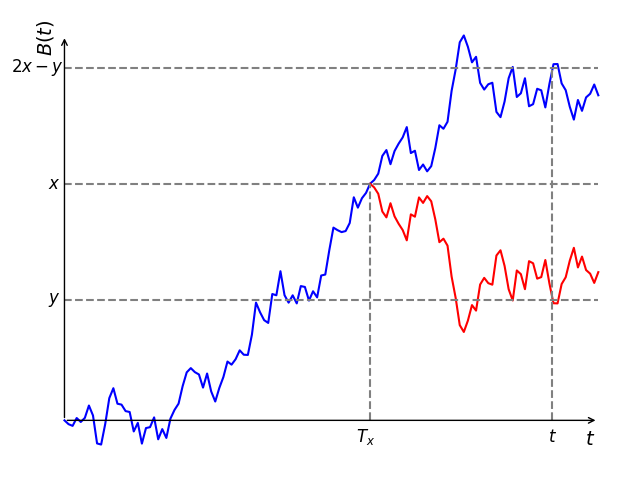
\includegraphics[scale=0.7]{figures/brownian_motion_symmetry_2.png}
    \caption{Brown 运动在首中时后的对称性 (2)}
    \label{fig:8.4.1}
\end{figure}

接下来介绍漂移 Brown 运动。

\begin{definition}\label{def:8.4.1}
    称一个随机过程 $\{X(t),t\geq0\}$ 为\emph{漂移 Brown 运动},若其满足:
    \begin{enumerate}
        \item $X(0)=0$
        \item $\{X(t),t\geq0\}$ 有平稳增量性和独立增量性
        \item $\forall t\geq0,X(t)\sim N(\mu t,\sigma^2t)$
    \end{enumerate}
    其中 $\mu$ 和 $\sigma^2$ 分别为\emph{漂移系数}和\emph{方差参数}。
\end{definition}

满足 $X(t)\sim N(\mu t,\sigma^2t)$ 的漂移 Brown 运动也可由令 $X(t)=\sigma B(t)+\mu t$ 得到。有 $\mathrm E(X(t))=\mu t,\mathrm{Var}(X(t))=\sigma^2t,X(t)-X(s)\sim N(\mu(t-s),\sigma^2(t-s)),\forall0\leq s<t$。

最后介绍几何 Brown 运动。

\begin{definition}\label{def:8.4.2}
    若 $\{X(t),t\geq0\}$ 为漂移 Brown 运动,令 $Y(t)=e^{X(t)}$,则称 $\{Y(t),t\geq0\}$ 为\emph{几何 Brown 运动}。
\end{definition}

由定义知,若 $Y(t)$ 为几何 Brown 运动,则 $\log Y(t)$ 为漂移 Brown 运动。设 $\log Y(t)=\mu t+\sigma B(t)$,则 $Y(t)=e^{\mu t+\sigma B(t)}$,有 $Y(0)=1,\forall0\leq s<t,\mathrm E(Y(t)|Y(u)(0\leq u\leq s))=\mathrm E(e^{X(t)}|X(u)(0\leq u\leq s))=\mathrm E(e^{X(t)-X(s)}e^{X(s)}|X(u)(0\leq u\leq s))=e^{X(s)}\mathrm E(e^{X(t)-X(s)})=e^{X(s)}e^{\mu(t-s)+\frac12\sigma^2(t-s)}=Y(s)e^{\mu(t-s)+\frac12\sigma^2(t-s)}$,即 $Y(t)$ 也具有 Markov 性。但需要注意其没有独立增量性。令 $s=0$,得 $\mathrm E(Y(t))=e^{\mu t+\frac12\sigma^2t},\mathrm{Var}(Y(t))=\mathrm E(Y(t)^2)-\mathrm E^2(Y(t))=e^{2t(\mu+\sigma^2)}-e^{t(2\mu+\sigma^2)}$。

\begin{example}
    记 $Y_n$ 为某股票在 $n$ 时刻的价格,其收益率 $\frac{Y_n-Y_{n-1}}{Y_{n-1}}=\frac{Y_n}{Y_{n-1}}-1$,记 $X_n=\frac{Y_n}{Y_{n-1}}$,合理假设 $X_n$ 独立同分布,且 $\mathrm E(\log X_n)=\mu,\mathrm{Var}(\log X_n)=\sigma^2$,若 $Y_0=1$,则 $Y_n=\prod_{i=1}^nX_i$,故 $\log Y_n=\sum_{i=1}^n\log X_i$。根据 CLT,$\log Y_n$ 近似服从 $N(n\mu,n\sigma^2)$,近似为漂移 Brown 运动,故 $Y_n$ 近似为几何 Brown 运动。
\end{example}

\end{document}
